\section{Project description}

\subsection{Background}

Rydberg atoms are characterized by a single valence electron in a highly excited electronic bound state (with principal quantum number $n \gg 1$) \cite{Gallagher1994}. These atoms have exagerated features, since many experimentally important properties scale as a high power of $n$: their physical size $a_{\mathrm{Ry}} \sim a_0 n^2$ (where $a_0$ is the Bohr radius), radiative lifetimes as $n^3$ and the dipole-dipole interaction between dufferent atoms as $n^4$. Their most widely used interaction is the Rydberg blockade \cite{Jaksch2000}, where an atom in the Rydberg state can supress the excitation of physically nearby atoms. This interaction can be turned on and off with very good contrast (12 orders of magnitude in coupling strength). The above properties allow for very efficient coupling of Rydberg states and have many uses in quantum information and quantum simulation (such as the recently observed entanglement between Rydberg atoms \cite{Wilk2010}). Rydberg atomic systems were extensively studied in the last decade, both single atoms and Rydberg ensemble properties. A detailed discussion about the current state of research can be found in a recent review paper \cite{Saffman2010}. Most Rydberg atomic experiments require sub-Doppler cooling and shielding from electromagnetic fields, since the Rydberg state is sensitive to shifts introduced by motion and external fields.

Another group of physical systems that is often compared to Rydberg atomic ensambles in terms of quantim computing potential is ion traps. They have a number of advantages, such as individual addressing, fast and high fidelity quantum gates, very long storage and coherence times \cite{Lucas2007}. A disadvantage is that the coupling between ions is through the Coulomb interaction, which is always present. The electronic structure of ions, however, is very close to those neutral atoms used in the Rydberg coupling experiments (single valence electron). It is then natural to ask how would ionic Rydberg systems behave?

A recent theoretical proposal \cite{Mueller2008} examined the possibility of Rydberg ions, and their while they inherit many properties from both trapped ions and Rydberg atoms, they have quanlitatively different interactions. This difference stems from the fact that the highly excited electron can be described as ``nearly free'', thus Rydberg ions in an ion trap behave as a composite system: a double-positively charged, heavy core and a highly delocalized electron (see Figure \ref{fig:iontrap}). The interaction between the ground state ions, Rydberg ions and the electromagnetic field of the trap can be described as a combination of charge-charge, charge-dipole, charge-quadrupole and dipole-dipole interaction (while trapped ions only exibit the first, Rydberg atoms the last contribution). The large variety of interactions and that many of them are tunable (by the trap electric field strength or by the choice of the Rydberg level $n$) makes potentially possible to create many different coupling schemes. The methods for Rydberg excition and interacton, proposed in \cite{Mueller2008}, can also have faster operation than the ones with neutral atoms (several hundred MHz instead of few MHz).

\begin{figure}
  \begin{center}
    \includegraphics[width=0.7\textwidth]{iontrap}
    \caption{Adapted from \cite{Mueller2008}, the shematic view of Rydberg ions in an ion trap, where $x_{ho}$ is the oscillator length of the ion core, $a_{\mathrm Ry}$ is the size of the Rydberg orbit, $\xi$ is the ion-ion separation. Typical experiments would have $x_{ho} \ll a_{\mathrm Ry} \ll \xi$ with $\xi \approx 5 \mu{\mathrm m}$.}
  \end{center}
  \label{fig:iontrap}
\end{figure}

These properties hint for the wide variety of uses for Rydberg ions. They can potentially become part of the standard trapped ion toolbox, realizing fast and high fidelity quantum gates. Also, they can become resources themselves for quantum information processing, or using the Rydberg blockade scheme to simulate interacting spin-systems. Using multiple ion species (as e.g. was done in the case of sympathetic cooling \cite{Home2009}) one can introduce different inhomogenities or potentials into the quantum simulation.

Most established ion trap groups seem to pursue advanced quantum gates, larger number of ions and large scale traps \cite{Kielpinski2002}. Since the Rydberg ion experiments require extran microwave and optical fields compared to the traditional ion trapping, it is likely that a new system built from the ground up with these experiments in mind would have an advantage over the modification of current traps.


\subsection{Research objectives}
The research objectives of this proposal are the following:
\begin{enumerate}
 \item Build up an ion trap experiment based on a species that is selected based on its qualities for Rydberg ion.
 \item Build up the mixed microwave-laser system that was theoretically proposed \cite{Mueller2008}, demonstrate Rydberg ion creation and then single-quibit manipulation.
 \item Demonstrate Rydberg blockade in the ion system, thus setting the way for two-qubit gates and entanglement.
 \item Parallel to the experimental effort, establish solid theoretical background for these systems, thus searching for other possible single- and two-ion manipulation methods.
\end{enumerate}


\subsection{Longer term outlook}
On the longer term these experiments should serve as foundations for a variety of potential further studies, some of them listed here as examples:
\begin{itemize}
 \item Testing different isotopes / ion species (with and without nuclear magnetic moment and thus hyperfine structure)
 \item Mixed ion systems for sympathetic cooling, selective excitation of qubits
 \item Mixed ion and Rydberg ion quantum computing (ions for information transport, Rydberg-type interaction for fast gates)
 \item Different trap geometry to test theoretical predictions about Ising-type spin chains (e.g. ring-trap \cite{Champenois2010} to implement the systems studied in \cite{Weimer2010})
\end{itemize}
